\documentclass{beamer}
\hypersetup{unicode}
\usepackage[utf8]{inputenc}
\usepackage[croatian]{babel}
\usepackage{csquotes}
\MakeOuterQuote{"}
\usepackage{thmtools}

\usepackage{datetime}
\newdate{date}{08}{06}{2024}
\date{\displaydate{date}}

\declaretheorem{teorem}
\declaretheorem[style=remark, sibling=teorem]{primjer}
\declaretheorem[style=remark, sibling=teorem]{napomena}
\declaretheorem[style=definition, sibling=teorem]{definicija}

\usepackage[style=authoryear]{biblatex}
\usepackage{tikz}

\usepackage{listings}


% manage colors: https://www.r-bloggers.com/2011/11/create-your-own-beamer-template/
% and https://ramblingacademic.com/2015/12/08/how-to-quickly-overhaul-beamer-colors/

\usetikzlibrary{arrows}
\newcommand{\midarrow}{\tikz \draw[-triangle 90] (0,0) -- +(.1,0);}

\definecolor{seagreen}{HTML}{21b2aa}
\definecolor{magenta}{HTML}{b2217f}
\definecolor{gold}{HTML}{ca9520}
\definecolor{red}{HTML}{da272f}
\definecolor{blue}{HTML}{4682b4}
\definecolor{purple}{HTML}{a65cef}

\definecolor{white}{HTML}{ffffff}
\definecolor{dwhite}{HTML}{eeeeee}
\definecolor{black}{HTML}{000000}
\definecolor{lblack}{HTML}{222222}

\colorlet{bgmain}{seagreen}
\colorlet{bgsec}{magenta}
\colorlet{bgter}{gold}
\colorlet{fgmain}{black}
\colorlet{fgsec}{lblack}

\usetheme{Madrid}
\usecolortheme{orchid}
% \useinnertheme{rounded}

\setbeamercolor{titlelike}{parent=structure, bg=seagreen, fg=white}
\setbeamercolor{palette primary}{bg=magenta, fg=white}
\setbeamercolor{palette secondary}{bg=magenta, fg=white}
\setbeamercolor{palette tertiary}{bg=magenta, fg=white}
\setbeamercolor{palette quaternary}{bg=magenta, fg=white}
\setbeamercolor{structure}{bg=white, fg=magenta} % itemize, enumerate, etc
\setbeamercolor{section in toc}{fg=black, bg=lblack} % TOC sections
\setbeamercolor{frametitle}{fg=white, bg=seagreen}

\setbeamercolor{block title}{fg=white, bg=seagreen}
% \setbeamercolor{block body}{bg=white, fg=white}

% Override palette coloring with secondary
\setbeamercolor{subsection in head/foot}{bg=seagreen,fg=white}

\lstdefinestyle{mystyle}{
	backgroundcolor=\color{white},
	commentstyle=\color{magenta},
	keywordstyle=\color{seagreen},
	stringstyle=\color{magenta},
	basicstyle=\ttfamily\footnotesize,
	breakatwhitespace=false,
	breaklines=true,
	captionpos=b,
	keepspaces=true,
	numbers=none,
	showspaces=false,
	showstringspaces=false,
	showtabs=false,
	tabsize=2
}
\lstset{style=mystyle}

\title[RS5]{Utjecaj distribucije podataka na vjerojatnost pokrivanja $t$-intervala pouzdanosti za sredinu populacije }
\subtitle{Projekt iz kolegija Računarska statistika (zadatak 5.)}
\author{Luka Šimek}
\institute[PMF--MO]{Prirodoslovno-matematički fakultet --- Matematički odsjek\\Sveučilište u Zagrebu}
\date{\today}

\begin{document}
% \nocite{*}

\begin{frame}[plain]
\titlepage
\end{frame}

\begin{frame}{Sadržaj}
\tableofcontents
\end{frame}

\section{Pojmovi}
\begin{frame}{Pojmovi}
\[
	\gamma_1 = \mathbb E \left( \frac{X - \mathbb E X}{\text{Var} X} \right)^3
	\quad \mathrm{i} \quad
	\gamma_2 = \mathbb E \left( \frac{X - \mathbb E X}{\text{Var} X} \right)^4-3
\]
\vskip 20pt

Ako je \( X \sim N(\mu, \sigma) \) i \( X_1, X_2, \ldots, X_n \)
slučajni uzorak, tada je 
\[
	\frac{\overline X_n - \mu}{S_n}\sqrt n \sim t(n-1),
\]
pri čemu je \( S_n \) uzoračka varijanca. Iz toga dobivamo 
pouzdani interval (\( t \)-interval) pouzdanosti \( 1-\alpha \) 
za sredinu populacije \( \mu \) kao
\[ \overline X_n \pm \frac{S_n}{\sqrt n}t_{\frac \alpha 2, n-1} .\]

	Pitanje: vrijedi li slični rezultat ako \( X \) nije
	normalno distribuirana?
\end{frame}

\section{Zadatak}
\begin{frame}{Parametri}
	MC studiju provodimo po kombinacijama faktora:
	\begin{itemize}
		\item duljina uzorka $n= 10, 15, 20, 50, 100$
		\item \( \gamma_1 = -2, 0, 2 \)
		\item \( \gamma_2 = 0, 6, 11 \)
		\item \( \mu=0, \sigma=5 \)
	\end{itemize}

	\vskip 30pt
	Za svaku trojku \( (n, \gamma_1, \gamma_2) \)
	simuliramo 500 uzoraka duljine \( n \). Na temelju
	njih procjenjujemo stvarnu vjerojatnost pokrivanja
	nominalno 90\%-p.i.\ i 95\%-p.i.
\end{frame}

\section{Rezultati}
\begin{frame}{Ovisnost o $n$}
	\begin{figure}
		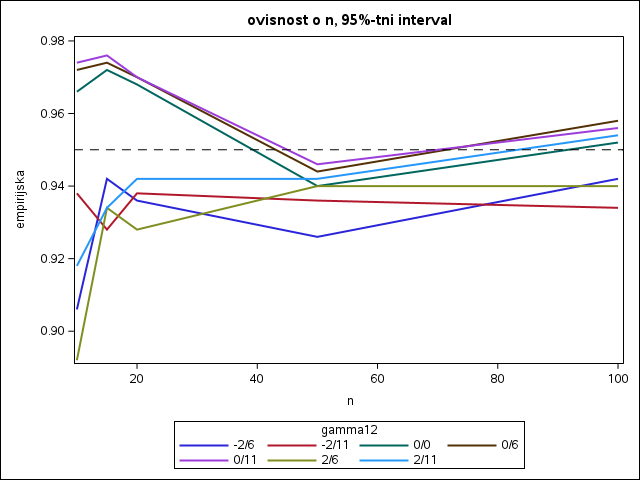
\includegraphics[scale=0.6]{assets/grafn95.png}
		\centering
		\caption{Ovisnost vjerojatnosti o \( n \) za fiksne \( \gamma_1, \gamma_2 \), 95\%-p.i.}
		\label{grafn95}
	\end{figure}
\end{frame}

\begin{frame}{Ovisnost o $\gamma_1$}
	\begin{figure}
		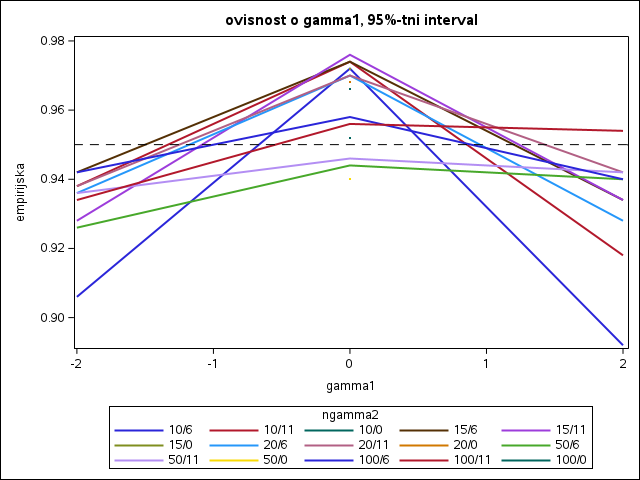
\includegraphics[scale=0.6]{assets/graf195.png}
		\centering
		\caption{Ovisnost vjerojatnosti o \( \gamma_1 \) za fiksne \( n, \gamma_2 \), 95\%-p.i.}
		\label{graf195}
	\end{figure}
\end{frame}

\begin{frame}{Ovisnost o $\gamma_2$}
	\begin{figure}
		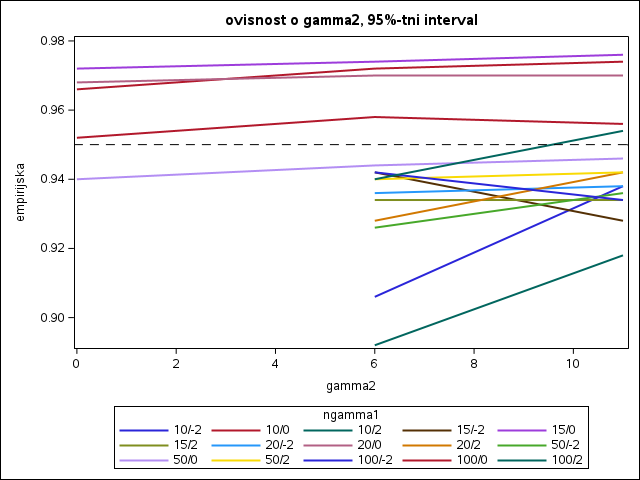
\includegraphics[scale=0.6]{assets/graf295.png}
		\centering
		\caption{Ovisnost vjerojatnosti o \( \gamma_2 \) za fiksne \( n, \gamma_1 \), 95\%-p.i.}
		\label{graf295}
	\end{figure}
\end{frame}

\begin{frame}{Zaključci}
	\begin{itemize}
		\item problematične su nesimetrične distribucije, naročito s malim uzorcima
		\item za simetrične spljoštene distribucije rezultati su slični kao za normalnu
	\end{itemize}
\end{frame}

\end{document}

